\documentclass[a4paper,twocolumn,10pt]{article}
\usepackage[spanish]{babel}
\usepackage[T1]{fontenc}
\usepackage[utf8]{inputenc}
\spanishdecimal{.}
\usepackage{lmodern}
\usepackage[a4paper]{geometry}
\usepackage{graphicx}
\usepackage{flushend}
\usepackage{wallpaper}
\usepackage{amsmath}
\usepackage{float}
\usepackage{colortbl}
\usepackage[normalem]{ulem}
\useunder{\uline}{\ul}{}

\begin{document}

\title{Ley de Inverso Cuadrado y Ley de Stefan-Boltzmann}
\author{ \\Aldo Aliaga, Benjamín Yapur, Fabian Trigo \\ \textit{Departamento de Física y Astronomía, Universidad de Valparaíso}}
\twocolumn[
  \begin{@twocolumnfalse}
    \maketitle
    \begin{abstract}
  
    \end{abstract}
  \end{@twocolumnfalse}\bigskip]

\vspace{2cm}

\section{Introducción}

\subsection{Ley de Inverso Cuadrado}
La ley de inverso cuadrado enuncia que una cantidad física específica es inversamente proporcional al cuadrado de la distancia a la fuente de esta cantidad física. Generalmente aplica a una cantidad conservada radiada uniformemente desde una fuente puntual en un espacio tridimensional. 

La densidad de las lineas de flujo es inversamente proporcional al cuadrado de la distancia de la fuente debido a que la radiación emitida cubre un área esférica que aumenta con el cuadrado del radio. Por este motivo la intensidad es inversamente proporcional al cuadrado de la distancia.

\subsection{Ley de Stefan-Boltzmann}
La Ley de Stefan-Boltzmann describe el la potencia irradiado por un cuerpo negro en función de su temperatura. Específicamente, enuncia que la la energía irradiada por unidad de área de un cuerpo negro es directamente proporcional a la cuarta potencia de la temperatura:
\begin{equation}
    R=\sigma T^4
\end{equation}
Siendo $\sigma= 5.670374*10^{(-8)} [\frac{W}{m^{-2}}K]$ la constante de proporcionalidad.

En este experimento se mide la energía térmica emitida por el filamento de tungsteno de una bombilla. Cuya temperatura es calculada a partir de la siguiente ecuación:
\begin{equation}
    T=\frac{R-R_{ref}}{\alpha R_{ref}}+T_{ref}
\end{equation}
Donde $R$ es la Resistencia del filamento en T, $R_{ref}$ es la resistencia del filamento a temperatura ambiente, $T_{ref}$ es la temperatura ambiente y $\alpha = 4.5*10^{-3} [K^{-1}]$ es el coeficiente de temperatura de la resistividad del filamento.


\section{Montaje Experimental}
\subsection{Herramientas}
\begin{itemize} 
\item Sensor de radiación.
\item Lámpara de Boltzmann.
\item Fuente de poder.
\item Multitesters y conexiones.
\end{itemize}

\subsection{Experimento 1: Ley de Inverso Cuadrado}
Primero se pegó a la mesa una cinta métrica para medir la distancia entre la lámpara de Boltzmann y el detector de radiación, procurando que estos queden alineados tanto en altura como en el eje de la cinta.

Luego se conecta el sensor a un voltímetro para medir la Radiación en miliVolts y la lámpara a la fuente de poder variando ligeramente el voltaje.

Para la toma de datos se enciende la lámpara aumentando el voltaje en la fuente de poder y se realizan mediciones de la radiación a distintas distancias. Después de cada medición se tapa el sensor para evitar que se caliente y se mide la radiación del ambiente.

\subsection{Experimento 2: Ley de Stefan-Boltzmann}
Para este experimento se midió la temperatura ambiente y la resistencia del filamento a esta temperatura ($R_{ref}$).
EL montaje es el mismo que en el experimento anterior pero con la adición de un voltímetro a la lámpara y un amperimetro entre la lámpara y la fuente de poder como se muestra en la figura.

\begin{figure}[H]
    \centering
    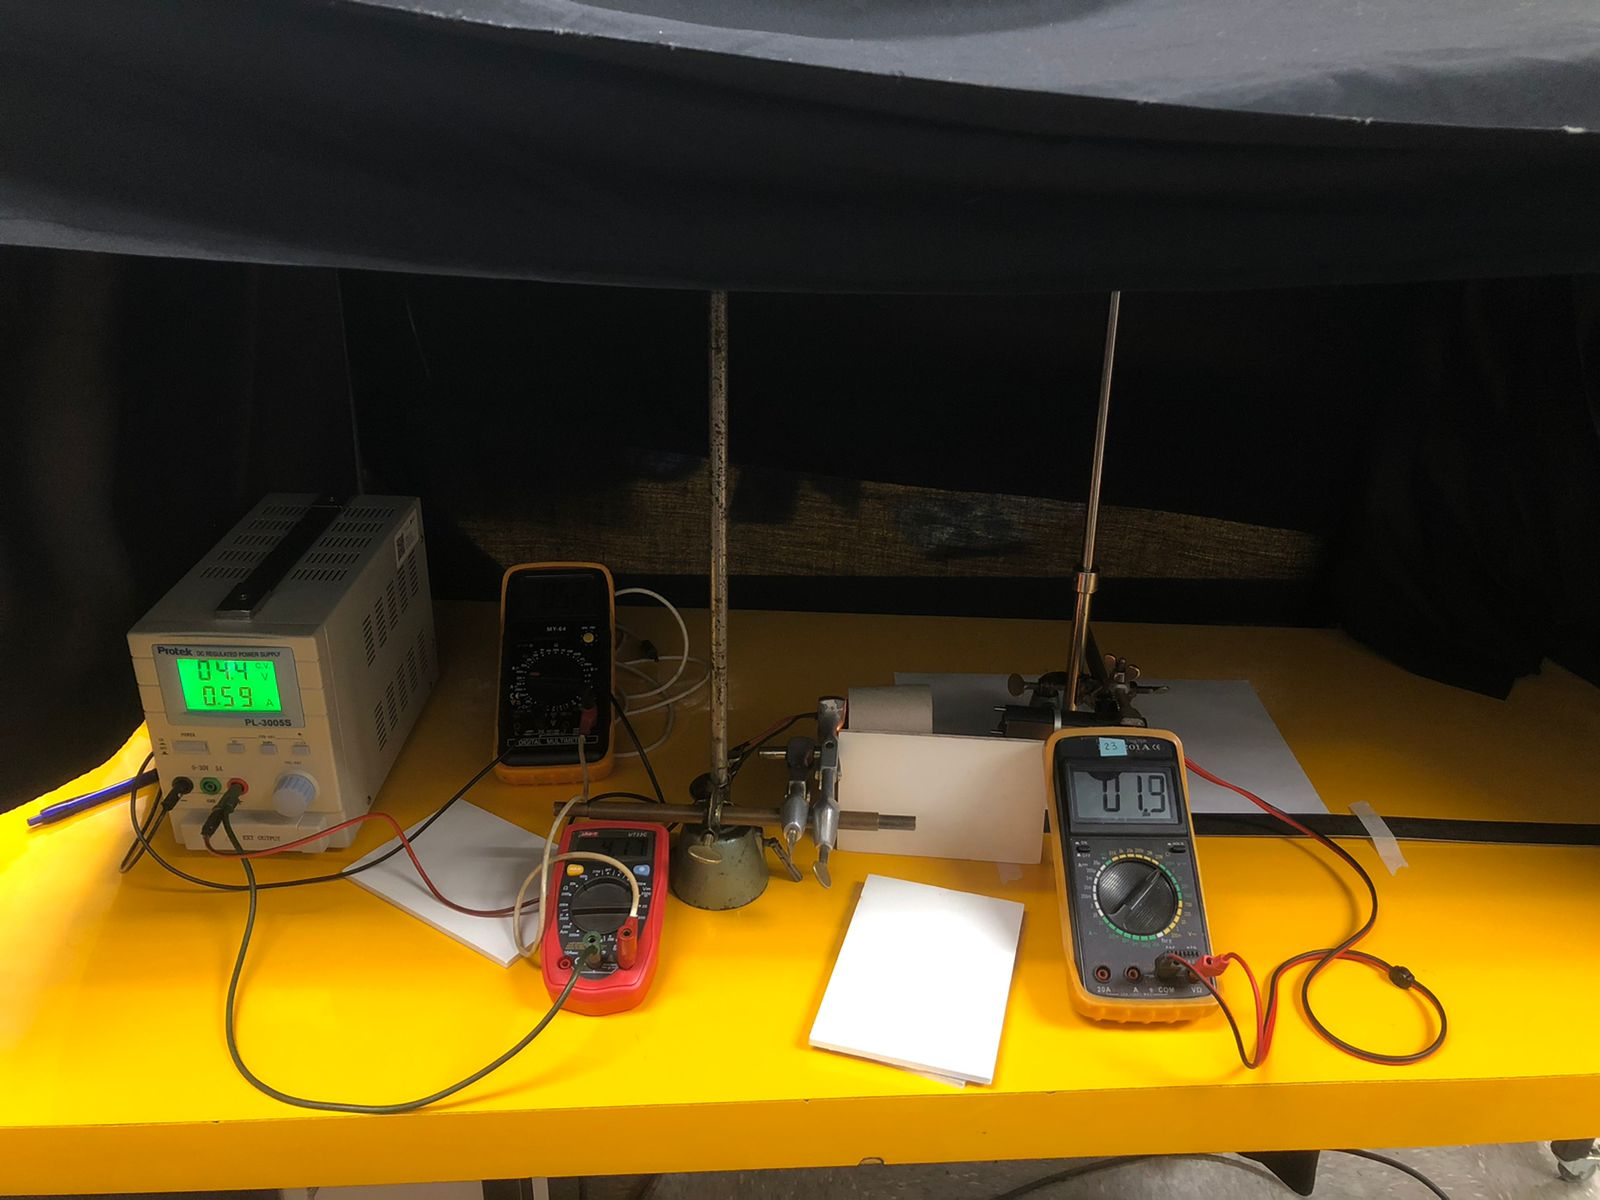
\includegraphics[scale=.12]{Imagenes/ISL_SB/montaje.png}
    \caption{Montaje del experimento.}
    \label{fig:my_label}
\end{figure}

De la misma forma se tomaron datos de la radiación para distintas distancias, así como el voltaje y corriente que fluye por la lámpara en cada medición.


\section{Análisis}



\section{Conclusión}
\section{Bibliografía}


\begin{itemize}
\item Wikipedia Contributors. (2022, August 27). Inverse-square law. Wikipedia; Wikimedia Foundation. https://en.wikipedia.org/wiki/Inverse-square law
\item Wikipedia Contributors. (2022, November 8). Stefan–Boltzmann law. Wikipedia; Wikimedia Foundation. https://en.wikipedia.org/wiki/Stefan%E2%80%93Boltzmann_law

‌

\end{itemize}


\end{document}

